\documentclass{scrartcl}
\usepackage[top=3cm, bottom=3cm, left=2cm,right=2cm]{geometry} 

\usepackage[english]{babel}
\usepackage[utf8]{inputenc}
\usepackage{mathtools}
\usepackage{esvect}
\usepackage{amssymb}
\usepackage{amsmath}

\usepackage{dcolumn}
\usepackage{booktabs}
\usepackage{tikz}
\usepackage{graphicx}
\usepackage{multicol}
\usepackage{float}
\usepackage{url}


\DeclareMathOperator*{\argmin}{argmin} % no space, limits underneath in displays
\DeclareMathOperator*{\argmax}{argmax} % no space, limits underneath in displays

\DeclarePairedDelimiter\abs{\lvert}{\rvert}%
\DeclarePairedDelimiter\norm{\lVert}{\rVert}%

\usepackage{titlesec}
\newcommand{\sectionbreak}{\clearpage}

\usepackage[parfill]{parskip}
\parskip = 4pt

\title{Pattern Analysis - Lecture notes}
\author{Sebastian Rietsch}

\begin{document}
\maketitle
\section{Random Forests}
\textit{What is a random forest?} An ensemble of decision trees.

\textit{What is a decision tree?} A binary tree with a "decision" at every internal and the root node. It is a learning based approach: A good decision functions at the internal nodes are the result of training.

\textit{What is a decision?} For example the answer to the question: "Is this sample on the right side of a hyperplane?"

\textit{Why an ensemble of trees?} Experience showed that it is complicated to train a single, highly accurate decision tree. The idea of random forests is therefore to train a large number of individually less accurate trees in a ranomized fashion, and to report then an averaged result of this forest. 
If we have a trained decision tree, we can test it by evaluating at the root node a function
\[h(\vec{x}, \vec{\vartheta}_j): \mathbb{R}^d \times \underset{\text{tree parameters}}{\mathcal{T}} \rightarrow \{0, 1\}.\]

Depending on the result we evaluate the test function at either the left successor or the right successor of the root node, and continue down the tree recursively until a terminal/leaf node is reached.
The leaf node performs an application-specific action. For example, if the task is to perfom classification, it assigns a label to the sample.

\textit{Training:} compute the tree parameters \(\vartheta\), consisting of
\begin{itemize}
    \item
        the tree height/depth (\textit{Note:} deeper trees tend to overfitt, must be complemented with increased number of trees, trade-off)
    \item
        the splitting function at each internal node
    \item
        if necessary, the "action" in the leaf node
\end{itemize}

It is important to note that this "binary tree paradigm" essentially performs a partitioning of the feature space. More specifically, each internal node subdivides the incoming samples into two parts.

\subsection{Specific task: classification}
Training of a single tree in a forest of size T
\begin{itemize}
    \item
        decide for a set of splitting function prototypes, e.g. hyperplanes or conics, ... (simpler functions are typically prefered. Simplest function: "axis aligned split")
    \item
        (decide for randomization)
    \item
        to find the parameters for the split function, select a suitable \underline{objective function}. 
\end{itemize}
"Solid choice": Information Gain
\[I = H(S_j) - \sum_{i \in \{L,R\}} \frac{\abs{S^i_j}}{\abs{S_j}} H(S^i_j)\]
where \(S_j\) is the data that flows into the node, \(S^L_j S^R_j\) is the data that flows to the left/right successor and \(H(\dots)\) denotes the entropy. (\textit{Note:} \(I = H_{\text{before}} - H_{\text{after, weighted}}\))
\[H(S_j) = -\sum_{c \in C} p(c) \cdot log(p(c)))\] 
where \(c\) denotes the class label, and \(p(c)\) the empirical distribution computed from \(S_j\). 

%Binary entropy function plot
\begin{figure}[ht]
	\centering
    \includegraphics[scale=0.5]{img/entropy.png}
	\caption{Binary entropy function}
	\label{fig:entropy}
\end{figure}



The candidate functions, out of which the best on is chosen with the information gain, are \underline{randomly drawn}. Typically, one decides:
\begin{itemize}
    \item
        how many candidate functions are drawn
    \item
        if also linear projection of the data shall be drawn (e.g. consider only dimensions \(\{d_{i_1}, d_{i_2}, \dots, d_{i_n}\}\)
    \item
        how the splitting parameters are sampled
\end{itemize}
\(\Rightarrow\) Note that a sparser sampling leads to more "noise"/less optimal results. (\textit{Note:} might be desired, e.g. prevents overfitting)

Choice of tree depth:
\begin{itemize}
    \item
        set maximum depth ("mandatory")
    \item
        optional: set minimum number of samples for split 
    \item
        depending on the application, stop if for example 99\% of features in a node belong to one class
\end{itemize}

Final classifier output:
\begin{itemize}
    \item
        at a leaf node, report the relative frequencies of the class labels in that node (e.g., 15\%: class 1, 85\% class 2)
    \item
        combine al trees by averaging the individual tree outputs. If a single discrete label is required, decide for the class with maximum probability.
\end{itemize}

\section{Random Forests 2}
Example: Classification
\begin{enumerate}
    \item
        Randomly select a number of splitting functions 
    \item
        Evaluate the information gain for each splitting function
    \item
        Set the function with maximum information gain as the current nodes' decision function
    \item
        Recursively repeat for the child nodes, until max tree depth (or some other criterium) is reached 
\end{enumerate}

\subsection{Regression Forests}
Goal: predict a \underline{continous} label \(p(y|\vec{x})\). (Remark: choice of the model complexity is related to the bias/variance trade off)

"Leaf prediction model": a base function that is fitted to the samples. The leaf prediction model could be
\begin{multicols}{2}
\begin{itemize}
    \item
        constant
    \item
        linear
    \item
        polynomial
    \item
        ...
\end{itemize}
\end{multicols}

To faithfully represent all of the data with a single function, it would certainly make sense to use a polynomial model, or something even more complex. However, the random idea implies to subdivide/partition the space, and to fit simpler models to the individual partitions. As a specific example, let's split up our input data points:

\begin{figure}[ht]
	\centering
    \includegraphics[height=4cm]{img/rf_regression.jpg}
	\caption{Regression split}
	\label{fig:rf_regression}
\end{figure}

The decision criterion for the splitting function works analogously to the classification case. The only difference ist that we need to define the entropy \(H(S_j)\) on continous values:
\[H(S_j) = -\frac{1}{\abs{S_j}} \cdot \sum_{\vec{x} \in S_j} \int_y p(y|x) \cdot log(y|x)dy\]
where \(p(y|x)\) can, e.g. be chosen as a Gaussian distribution \(p(y|x) = \mathcal{N}(y; \overline{y}(x), \sigma_y^2(x))\), where \(\overline{y}(x)\) is a linear function and \(\sigma_y(x)\) is the conditional variance computed from a linear fit.

%Probabilistic linear fit:
%\begin{figure}[H]
%	\centering
%    \includegraphics[height=4cm]{img/rf_linearfit.jpg}
%	\caption{Probabilistic linear fit}
%	\label{fig:rf_regression}
%\end{figure}

Combining the expression for \(p(y|x)\) into \(H(S_j)\) yields
\[H(S_j) = \frac{1}{\abs{S_j}} \cdot \sum_{\vec{x} \in S_j} \frac{1}{2} \cdot log((2 \pi e)^2 \sigma_y^2(\vec{x}))\]
\[\Rightarrow I(S_j, \vartheta) = \sum_{\vec{x} \in S_j} log(\sigma_y(\vec{x})) - \sum_{i \in \{L, R\}} (\sum_{x \in S_j^i} log (\sigma_y(\vec{x}))) \]

\subsection{Density Forests}
Very same idea, adapted to unlabelled data $\Rightarrow$ learning-baed density estimator.

Each leaf node is modeled as a multivariate Gaussian distribution. The information gain metric can again be reused, i.e. \(I(S_j, \vartheta) = H(S_j) - \sum_{i \in \{L, R\}} \frac{\abs{S_j^i}}{\abs{S_j}} \cdot H(S_j^i)\) but let us choose \(H(S_j)\) as
%Fancy
\[
H(S_j) = \frac{1}{2} \cdot log((2 \pi e)^d \abs{
    \underset{\mathllap{
        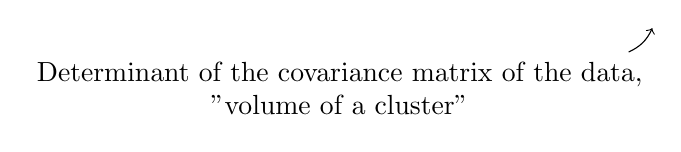
\begin{tikzpicture}
            \draw[->] (-0.3, 0) to[bend right=20] ++(0.3,2ex);
            \node[below left,align=center] at (0,0) {Determinant of the covariance matrix of the data,\\ "volume of a cluster"};
        \end{tikzpicture}
    }}{\Lambda} 
S_j})
\]

Plugging \(H(S_j)\) back into \(I(S_j, \vartheta)\) yields
\[I(S_j, \vartheta) = log (\abs{\Sigma(S_j)}) - \sum_{i \in \{L, R\}} \frac{\abs{S_j^i}}{\abs{S_j}} \cdot log(\abs{\Lambda(S_j^i)})\].

In each leaf, fit a multivariate Gaussian distribution to the data in that leaf using, e.g. MLE.

Note that the fitted densities have discontinuities at the splitting boundaries (this is the same type of discontinuity that we observed for regression forests or classification forests). However, remember that the result of a random forest is averaged over all individual trees. Because of randomization, each tree splits at a slightly different location, and thus the discontinuities are "averaged out" in the forest.
    
\section{Hidden Markov Models and Random Markov Fields}
Generative vs. Discriminative Model: let \(x\) denote the input, \(y\) the hidden variable/prediction/...
\[p(x,y) \Leftrightarrow p(y|x)\]

In a generative model, the available information is "more complete", i.e. we can for example also generate new samples \(x\) by sampling from \(p(x,y)\) by marginalizing over \(y\).

A discriminative model is slimmer (which is particularly useful for robust training with limited training data (the situation we're almost always in)); however, it only allows to discriminate between different \(y\)'s, but we can not generate new values \(x\).

\subsection{Remarks about HMMs}
\begin{itemize}
    \item
        Probabilistic, graphical model
    \item
        the directed edge in the graph can be understood as a statistical dependency: \[S_1 \rightarrow S_2 \Rightarrow p(S_2|S_1)\]
    \item
        Generative approach
    \item
        For many tasks, including speech processing, we oftentimes only allow for state transitions \(a_{ij}\) with \(i \leq j\). (no backward links) Those restricted HMMs are called "Left-right HMMs", as opposed to fully connected ("ergodic") HMMs.
\end{itemize}

\medbreak
How can we generate observations with an HMM?
\begin{enumerate}
    \item
        Sample from \(\pi = (\dots)\) (this gives you starting state) 
    \item
        Let \(S_1\) denote the starting state. Sample from \(b_1\) (column or row from production probability matrix \(B\)) a symbol
    \item
        Sample from \(\vec{a}_{S_1}\) (column or row from state transition matrix \(A\)) the next state
    \item
        Repeat 2.-3. until (randomly drawn/desired) word length reached
\end{enumerate}

\subsection{Markov Random Fields (MRF)}
1985, Geman/Geman: introduced MRFs to image processing:  Consider the pixel grid as a lattice (Gitter) of random variables.

More specifically, let us assume that the image \(F\) is given by the random matrix \([f_{ij}]\). %\(\Rightarrow p([f_{ij}])\). 

Assumption: limited statistical dependency:
\[p(f_{ij}| f_{i-1, j-1}, f_{i, j-1}, f_{i-1,j})\]
where \(f_{i-1, j-1}, f_{i, j-1}, f_{i-1,j})\) form a dependency of the neighbors to \(f_{i,j}\) (This will be our Markov property).

\[p([f_{ij}]) = \prod_{i,j} p(f_{i,j} | f_{i-1, j-1}, f_{i, j-1}, f_{i-1,j})\]

\subsubsection{Definition of MRF}
Lets us consider the features/observations \(\vec{x}_1,\vec{x}_2, \dots, \vec{x}_N\)
\begin{enumerate}
    \item
        Positivity: \(p(\vec{x}_1,\vec{x}_2, \dots, \vec{x}_N) > 0\)
    \item
        Markov property: \(p(\vec{x}_k | \vec{x}_1, \dots, \vec{x}_{k-1},\vec{x}_{k+1} \dots, \vec{x}_N) = p(\vec{x}_k|\mathcal{N}(\vec{x}_k))\) where \(\mathcal{N}(\vec{x}_k)\) denoted the neighborhood of \(\vec{x}_k\).
\end{enumerate}
Definition of the neighborhood: 
\begin{enumerate}
    \item
        \(\vec{x}_k \notin \mathcal{N}(\vec{x}_k)\)
    \item
        \(\vec{x}_i \in \mathcal{N}(\vec{x}_k) \Rightarrow \vec{x}_k \in \mathcal{N}(\vec{x}_i)\)
    \item
        \(\mathcal{N}(\vec{x}_k) = \{\vec{x}_i | 0 < dist(\vec{x}_i, \vec{x}_k) \leq t\}\)
\end{enumerate}
Example: Pixel grid:
\(\mathcal{N}(\vec{x}_{i,j}) = \{x_{k,l} | (i - k)^2 + (j - l)^2 \leq c^2, i \neq k \text{ or } j \neq l \}\)
\begin{itemize}
    \item
        NESW as neighbors, 4-Neighborhood \((c=1)\)
    \item
        All around as neighbors, 8-Neighborhood \((c=\sqrt 2)\)
\end{itemize}

\section{Markov Random Fields (continued)}
(Graph) clique: Complete subgraph

Gibbs Random Field (GRF): A GRF is given by the PDF 
\(p(x) = \frac{1}{
\underset{\mathllap{
        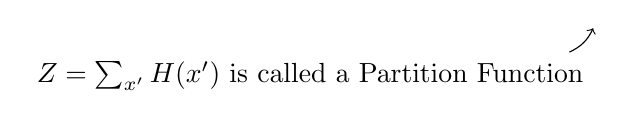
\begin{tikzpicture}
            \draw[->] (-0.3, 0) to[bend right=20] ++(0.3,2ex);
            \node[below left,align=center] at (0,0) {\(Z = \sum_{x'}H(x')\) is called a Partition Function};
        \end{tikzpicture}
    }}{Z}}  e^{-H(x)}\)
, where \(H(x)\) is an energy function, i.e. a sum of potential functions. For a given PDF \(p(x)\), the choice of energy function is not unique. Consider for example:
\[H(x) = - log p(x) - log Z \]
\[p(x) = \frac{1}{Z} e^{-H(x)} = \frac{1}{Z} e^{log p(x)} e^{log Z} = p(x)\]
\[\Rightarrow \text{we can chose Z arbitratily}\]

The interesting theoretical property is that GRF and MRF are equivalent. This is called the \textit{Hammersley-Clifford Theorem}.

\bigbreak

\subsection{Example: image denoising}
Given: Observed noisy image \([g_{ij}]\)

Hidden variables are the ideal (noiseless) images \([f_{ij}]\).

\textbf{Assumption 1:} the ideal image is spatially smooth \[p([f_{ij}]) = \frac{1}{Z} \cdot e^{-H([f_{ij}])}\] where \(H([f_{ij}]) = \sum_{ij} \norm{\Delta f_ij}_2^2\) (sum of squared gradients, computed over a neighborhood) (Note: Smoother image produces smaller \(H\), which maximizes \(p([f_{ij}])\).

\textbf{Assumption 2:} \([g_{ij}]\) is similar to \(f_{ij}\), but corrupted by additive Gaussian noise.
\[ p([g_{ij}]|[f_{ij}]) = \prod_{i,j} \frac{1}{\sqrt{2\pi} \sigma_{ij}} \cdot exp(-\frac{1}{2\sigma_{ij}^2} \cdot \underset{\text{energy function H}}{(f_{ij} - g_{ij})^2)}\]

With these two functions defined, we can solve for a MAP estimte for \(f\): 
\begin{align*}
    \underset{\text{estimated ideal image}}{[\hat{f}_{ij}]} &= \argmax_{[f_{ij}]} p([f_{ij}]|[g_{ij}])\\
    &= \argmax_{[f_{ij}]} p([g_{ij}]|[f_{ij}]) \cdot p([f_{ij}])\\
    &= \dots \text{(take log)}\\
    &= \argmin_{[f_{ij}]} \{\sum_{ij} \norm{\Delta f_{ij}}_2^2 + \sum_{ij} \lambda_{ij}(f_{ij} - g_{ij})^2\}
\end{align*}
\(\norm{\Delta f_{ij}}_2^2\): function of clique of size 2

Lecture slides: \url{https://www.slideshare.net/ykwang/markov-random-field-mrf} 
\end{document}
